\documentclass[conference]{IEEEtran}
%Template version as of 6/27/2024

\usepackage{cite}
\usepackage{amsmath,amssymb,amsfonts}
\usepackage{algorithmic}
\usepackage{graphicx}
\usepackage{textcomp}
\usepackage{xcolor}
\def\BibTeX{{\rm B\kern-.05em{\sc i\kern-.025em b}\kern-.08em
    T\kern-.1667em\lower.7ex\hbox{E}\kern-.125emX}}
\begin{document}

\title{Exploring AI Agent Systems and Orchestration}

\author{Natalie Lambert}

\maketitle

\begin{abstract}
Artificial intelligence agent systems driven by Large Language Models (LLMs) 
have evolved from simple zero-shot prompting into complex single-agent and multi-agent workflows
capable of multi-step problem solving, with minimal human intervention.
As LLM capabilities plateau in zero-shot performance, 
AI agent systems increasingly rely on orchestration techniques and execution constraints
to successfully complete tasks.
This survey explores the evolving landscape of agentic architectures, contrasting single-agent systems 
with multi-agent paradigms. 
This work examines important aspects of agentic design, such as workflow coordination, 
communication protocols, context management, system scalability and costs, benchmarks and reliability. 
Finally, the paper highlights key open challenges and opportunities from a systems perspective,
advocating for principled, constraint-guided designs to build reliable and cost-effective agent deployments.
\end{abstract}

\begin{IEEEkeywords}
artificial intelligence, multi-agent, single agent, orchestration, benchmark, context, reliability.
\end{IEEEkeywords}

\section{Introduction}\label{intro}
AI agent systems is a branch of artificial intelligence research that examines how
models can be harnessed to exhibit emergent reasoning and step-by-step problem-solving, given a
specific input task definition.
These systems are said to have \emph{agency} if there is little to no human involvement while the
system plans and executes the task at hand.
Although it is possible to harness any kinds of models in this way, the most prominent real-world
example is the application of AI agent systems that use Large Language Models (LLMs),
where a user inputs a natural language description of a task (called a prompt), and receives the
final result once the agent system has executed to completion.

Agentic architecture are ways in which LLMs and auxiliary tools can be organized, in order to allow
for a structured definition of how LLMs can interact with inputs and the surrounding environment.
Organizing and restricting how an LLM is allowed to process information and complete tasks acts as a
way to secure the system, so that the LLM cannot execute arbitrary steps that may be destructive.
Architectural decisions involve deciding how many of which kind of model are part of the system, how
resources are allocated between models, and which tools (e.g. for writing code, accessing local
files or browsing the Internet) are available.

Agent orchestration refers to the control layer that manages aspects such as task delegation,
data sharing, system state management and inter-agent communication.
In tandem with the structural definitions of the system architecture, orchestration implements the
actual processes that make an agentic system functional.
This constraint-focused perspective of AI agents has emerged from a trend towards the use of
so-called \emph{hybrid} systems, which borrow concepts and merge implementations of classical symbolic
AI frameworks and generative neural systems \cite{ali_agentic_2025}.
Since generative AI are inherently probabilistic in nature, they pose challenges in terms of
reproducibility and interpretability.
On the other hand, symbolic AI systems are rule-based, and are thus too inflexible to new workloads.
A common approach in designing agentic systems has been to incorporate aspects of both types of AI
systems, to provide an advantageous middle-ground in terms of adaptability and reliability.

\subsection{Motivation and Background}
As foundational models plateau in zero-shot capabilities, researchers look to agent orchestration
techniques as a promising approach for improving task solving accuracy.
The design principles that determine how an agentic system can be improved remain underexplored,
causing real-world deployments to rely heavily on empirical heuristics and ad hoc decisions
rather than principled, robust design and implementation \cite{kim_towards_2026}. 
Some of the key research questions in agent system development include: 
\begin{itemize}
	\item Do agent architectures (which provide scaffolding around LLMs) add inherent constraints to the
		system, preventing drift and keeping the LLM focused on accurate task completion?
	\item How do AI agents prevent silent error propagation? 
	\item What are the true cost-latency trade-offs of scaling an agentic system from one LLM to
		several communicating models? 
	\item How can hybrid approaches (e.g. in agent architecture patterns, tool use management)
		facilitate more flexible systems? 
	\item Assuming the underlying LLMs are treated as blackboxes, is it possible to build systems
		that do not rely on a deep knowledge of the model internals, and yet are able to achieve
		both reasonable accuracy and reliability?
\end{itemize}
Understanding these systems is foundational for solving tasks that require
sustained multi-step interactions, iterative information gathering under partial observability,
and adaptive strategy refinement \cite{kim_towards_2026}.

\section{Agent System Architectures}
Agentic systems have much in common with distributed systems, in that architectures are often composed 
of modular building blocks that have a clear interface for passing prompts, LLM responses and tool outputs. 
Understanding how an agentic system works hinges on examining the interaction of its modules,
and reasoning about how each individual component impacts the overall system.

Two categories of agentic architectures have emerged and are widely adopted.

\subsection{Single Agent Systems}
A single agent system is composed of a single LLM, surrounded by a minimal harness which allows for
tool-calling capabilities and iteration (Fig.~\ref{fig-sas}).
Despite the use of enhancements such as Retrieval Augmented Generation (RAG)
and the Model Context Protocol (MCP), Single Agent Systems (SAS) are not able
to solve tasks that are beyond a certain complexity,
since the context window of the central LLM is constrained \cite{gao_single-agent_2025, patel_dynamic_2026}.
While defining these tasks and categorizing the complexity is an open issue yet
to be fully addressed or quantified by an agentic benchmark, Single Agent Systems (SAS) 
are primarily used in the context of sequential tasks where maintaining a linear chain of thought 
is necessary \cite{kim_towards_2026}.

\begin{figure}[htbp]
\centerline{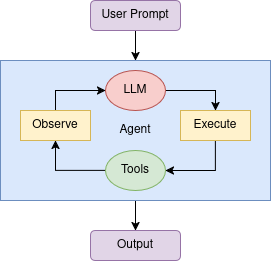
\includegraphics[width=1.75in]{figs/SAS.png}}
\caption{A schematic showing the main components of a single agent system.}
\label{fig-sas}
\end{figure}

Furthermore, single agents struggle with data-intensive reasoning. 
In evaluations like LiveAgentBench, which tests agents against real-world web challenges across domains such 
as humanities, law, and economics, the best agents' accuracy score was 35\% compared to a 70\% human baseline, 
although the use of tool calls provided a 56\% boost over isolated LLMs \cite{li_liveagentbench_2026}. 
Moreover, a agent shows a tendency towards context drift (which leads to unhelpful hallucinations),
infinite loops, or a premature halt without completing the assigned task.

\subsection{Multi-Agent Systems}
A Multi-Agent System (MAS) is composed of two or more single agents that interact, which results in
a system that can decompose and parallelize tasks.
The literature identifies several structural organizations and collaboration strategies 
for MAS, ranging from pure cooperation to adversarial debate and competition
\cite{yarmohammadtoosky_llm-powered_2026}.

Current MAS architectures face severe coordination complexities and scalability issues 
\cite{yarmohammadtoosky_llm-powered_2026}. 
One of the most pronounced problems is topology-dependent error amplification. 
In completely independent multi-agent systems, unchecked error propagation results in up to 17x 
more errors than a single-agent baseline \cite{kim_towards_2026}. 
Even when a centralized \emph{orchestrator} agent (synonymous with central manager agent) 
is introduced to check errors, the error rate is still 4x that of the baseline, 
and the system suffers from a validation bottleneck at the orchestrator \cite{kim_towards_2026}.
Moreover, the existence of a central leader agent node leads to a performance bottleneck, since
all sub-agents must wait for the leader agent to arbitrate and resolve inconsistencies in sub-task
completion.
To mitigate logical inconsistency, duplicate operations, and unbounded autonomy, 
robust coordination layers are strictly required \cite{adimulam_orchestration_2026},
but a key challenge with MAS is the difficult task of transmitting the right amount of context 
between agents: papers discuss the existence of a phenomenon called context fragmentation.

While MAS have shown promise in handling more complex task resolutions, the continued (although
slow) improvements in frontier LLMs cause the gap to narrow between SAS and MAS accuracy scores
\cite{gao_single-agent_2025}.
Thus, MAS are not a panacea: they exhibit \emph{capability saturation},
which means that if a single agent's base accuracy on a task exceeds 45\%, 
assigning multiple agents to the same task will generally incur higher coordination 
and compute costs than benefit gained from the increased accuracy score \cite{kim_towards_2026}.


\section{Workflow Coordination}
When there are multiple agents cooperating to solve a single task, it becomes necessary to define a
workflow for describing how each agent contributes, and how agents coordinate between themselves to
delegate sub-tasks and resolve conflicts or inconsistencies.
There are several paradigms for such systems, which have been tailored to solving particular task types.

\subsection{Independent Multi-Agent Systems}
Independent MAS refers to the simplest paradigm where multiple non-communicating agents solve tasks in
parallel, after which all the outputs are aggregated \cite{kim_towards_2026}.
These kind of systems are best used when it is desirable to include multiple diverse answers, but
they often require a subsequent deduplication step on the outputs.
However, for more data-driven or complicated tasks, independent MAS often under-perform compared to
more structured approaches \cite{taleb_expansion-contraction_2026}.

\begin{figure}[htbp]
\centerline{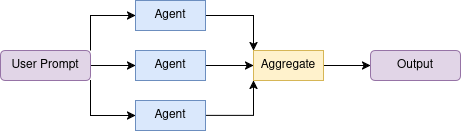
\includegraphics[width=2.75in]{figs/mas-indep.png}}
\caption{The structure of an independent multi-agent system.}
\label{fig-mas-indep}
\end{figure}

\subsection{Hierarchical Agent Systems}
Hierarchical, centralized, or layered, systems rely on top-down control where a 
higher-level orchestrator makes strategic decisions, manages dependencies, and 
delegates to worker, service, or support sub-agents \cite{yarmohammadtoosky_llm-powered_2026,
adimulam_orchestration_2026}.
This agent paradigm is naturally suited for tasks that are easily decomposable.

\begin{figure}[htbp]
\centerline{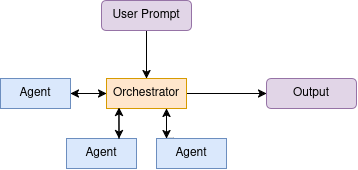
\includegraphics[width=2.5in]{figs/mas-centr.png}}
\caption{The organization of a hierarchical multi-agent system.}
\label{fig-mas-centr}
\end{figure}

Centralized agents often implement sub-agent management via a dynamic abstraction;
for example, AOrchestra treats sub-agents exactly as standard LLM tools. 
It introduces a framework-agnostic tuple (Instruction, Context, Tools, Model) 
that allows a central orchestrator to dynamically add, invoke, or remove sub-agents at runtime, 
achieving approximately 20\% performance improvement over a static system which only uses a static
sequencing of steps and pre-defined tool calls \cite{ruan_aorchestra_2026}.

Since a centralized agent is the defacto ``manager'' of the task completion process,
lifecycle management is a key concern. AgentOrchestra is a system that addresses lifecycle-aware 
coordination by deploying modular \emph{managers}, which are dedicated services that track
state changes, such as the Prompt Manager for prompt versions, the Dynamic Manager for code execution, 
and the global Version Manager to ensure complete traceability of system evolution
\cite{zhang_agentorchestra_2026}.

It is important to note that a centralized agentic system need not have a fixed number of sub-agents
throughout its operation.
Due to the large amount of context that an orchestrator needs to process,
there has been an exploration of how to use lazy-loading and just-in-time agent system adaptation,
which keeps only the most recently-used tool APIs, sub-agent descriptions and information loaded in
context, offloading extra tools and idle agents until they are loaded on-demand \cite{sampath_adaptive_nodate}.
This allows for flexibility in resource use, while maintaining the overall hierarchichal structure.

\subsection{Decentralized Networks of Agents}
Decentralized agentic systems distribute decision-making across a network of (mostly) 
independent agents \cite{yarmohammadtoosky_llm-powered_2026}. 
In decentralized MAS, an all-to-all peer-to-peer (P2P) communication is used, 
which removes centralized bottlenecks but makes synchronization highly expensive \cite{kim_towards_2026}. 
Similarly to centralized agents, decentralized agent systems are highly suited to decomposable
tasks, with the distinction that the inter-agent synchronization constraints must be relaxed to
allow for somewhat infrequent output exchanges.
An example of such a workflow would be an agentic debate, where individual agents come up with
different approaches to solving the task, and only exchange information when required to compare
outputs between themselves.

\begin{figure}[htbp]
\centerline{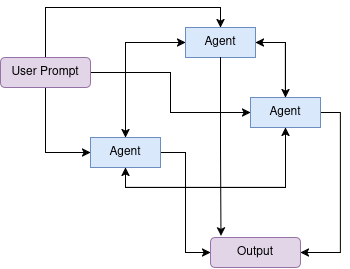
\includegraphics[width=2.25in]{figs/mas-decentr.png}}
\caption{A schematic of a decentralized network of agents.}
\label{fig-mas-decentr}
\end{figure}

\subsection{Agent Routing and Cascading}
The idea of leveraging two different systems depending on task difficulty pre-dates AI agents;
so-called \emph{routing of requests} has been employed for switching requests between an LLM and a
Small Language Model (SLM) to cut costs \cite{ding_hybrid_2024}.
A similar paradigm in the context of agentic systems is to choose between SAS or MAS
for a given task using one of two simple schemes \cite{gao_single-agent_2025}:
\begin{itemize}
	\item Routing: an LLM-as-judge, which is a secondary helper model, determines a complexity
		score for a task, and assigns the task to a MAS (if the task is of high complexity)
		or to a SAS (if the task is of low complexity) according to a user-defined threshold.
	\item Cascade: an SAS first attempts to solve a task. Upon failure, the task is redirected to a MAS.
\end{itemize}
Both workflow mechanisms allow for strategic selection of different model types, although in both
cases they are not necessarily optimal, since they function using a best-guess or retry heuristic.

\begin{figure}[htbp]
\centerline{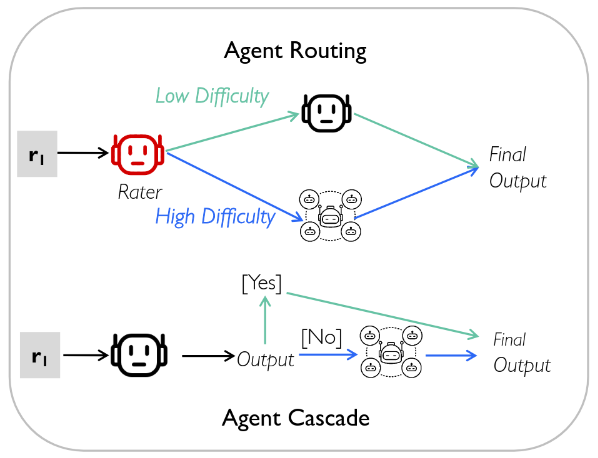
\includegraphics[width=2.5in]{figs/mas-routing.png}}
	\caption{Two schematics comparing agent routing (top) and agent cascade (bottom) from 
	\cite{gao_single-agent_2025}. $r_1$ stands for the input prompt.}
\label{fig-mas-routing}
\end{figure}

\subsection{Task Decomposition}
To process complex tasks, systems must decompose them while maintaining logical dependencies. 
The DynTaskMAS framework introduces a Dynamic Task Graph Generator that computes directed acyclic graph
(DAG) weights based on estimated task complexity and the estimated cost of information transfer \cite{yu_dyntaskmas_2025}. 
This DAG allows an Adaptive Workflow Manager and an Asynchronous Parallel Execution Engine to
optimize resource utilization using priority weights, claiming a 20-30\% decrease 
in execution times and near-linear scaling up to 16 agents \cite{yu_dyntaskmas_2025}.

\section{Agent Communication}
Inter-agent coordination becomes a necessity for most multi-agent systems, otherwise agents are
prone to the generation of duplicate or conflicting outputs.
However, for single agent systems, the communication overhead is non-zero, since LLMs now have
access to external resource in the form of tool call interfaces.
It has been measured that tasks which require a large amount of tool calls incur higher overall
multi-agent coordination, due to the compounding of multiple agents' actions \cite{kim_towards_2026}.
While there has been work that proposed novel coordination mechanisms, there is friction to maintain
the status quo with existing agent protocols, due to the expense of porting agentic applications to
a new interface.

\subsection{Protocols}
Standardized communication mechanisms remain a primary bottleneck for heterogeneous agent
interaction \cite{ehtesham_survey_2025}. 
However, to avoid fragmented and ad hoc integrations, several protocols have been widely adopted
\cite{ehtesham_survey_2025}:
\begin{itemize}
	\item Model Context Protocol (MCP): a standardized JSON-RPC client-server interface 
		designed strictly for tool invocation and typed data exchange.
	\item Agent Communication Protocol (ACP): a general-purpose RESTful HTTP protocol 
		that handles multi-part messages, session management, and routing, 
		making it ideal for long-running, stateful services.
	\item Agent Network Protocol (ANP): designed for open-network interactions over the internet, 
		allowing agents to securely discover each other using decentralized identifiers.
	\item Agent to Agent (A2A): enables peer-to-peer task delegation between agents,
		supporting secure and scalable collaboration.
		Each agent has its capabilities defined and available
		for peer agents to access when sending requests, although some work has shown that these
		natural language descriptions of functionality are not reliable \cite{smirnova_cost-aware_2026}.
\end{itemize}

AgentOrchestra provides a non-standard Tool-Environment-Agent (TEA) protocol, 
combining a version of ACP with a Tool Communication Protocol (TCP) and 
an Environment Communication Protocol (ECP) for end-to-end versioning and traceability
\cite{zhang_agentorchestra_2026}.

\subsection{Cache-to-Cache}
Cache-to-Cache (C2C) is a novel approach that challenges the need to use natural language
for inter-agent communication, since ambiguity, semantic equivalency and LLM internal biases cause
issues with reliable interpretation of text inputs by other LLMs
\cite{smirnova_cost-aware_2026, cox_mapping_2025, ali_agentic_2025}.
C2C allows for agents to share KV Cache values, which leads to zero output token cost for the source
agent (cutting down overall costs significantly), a 2.5 speed-up in latency, a 6-14\% increase in
accuracy, and a reduction in the token burden on the target agent.
However, the method is unusable if a weak model transfers its KV Cache values to a stronger model,
because the sharing mechanism merely leads to the addition of noise in the 
target agent's inputs \cite{fu_cache--cache_2025}.

\section{Context Management}
Effective context management is a key challenge that is central to LLMs in general, not just agentic systems.
Despite the increase in how much context can be handled by frontier models, recent research reveals
a discrepancy in how users perceive the additional available context, and what the actual trade-offs are.
For example, a phenomenon called the \emph{reasoning shift} occurs when a prompt is
padded with irrelevant context, shrinking the effective context by up to 65\% \cite{rodionov_reasoning_2026}.
The useless context triggers lazy behavior behaviour on the part of the LLM, which decreases the
amount of overall tokens spent on chain-of-thought reasoning and self-checking,
ultimately degrading accuracy on complex tasks.
This finding correlates with agentic systems inexplicably terminating early after
accumulating redundant and irrelevant context through many loop iterations over time.

Futhermore, experiments have demonstrated a drawback to extended context models, termed
the \emph{lost in the middle} phenomenon, which demonstrates that decoder-only models struggle
to retrieve information when the key text is sandwiched 
in the middle of a long context window (2-6K tokens),
exhibiting worse accuracy scores than closed-book baselines \cite{liu_lost_nodate}.
Accuracy scores are highest only when crucial details are placed at the very beginning or end of the context. 

\begin{figure}[htbp]
\centerline{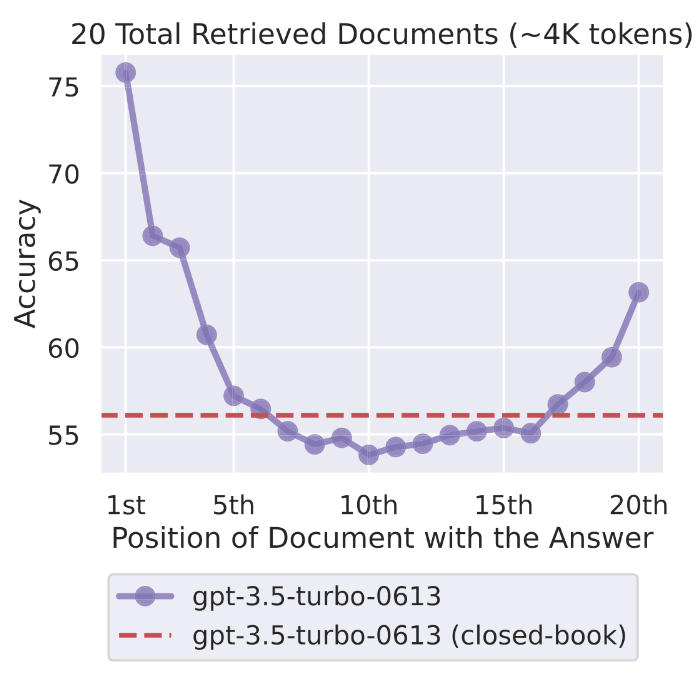
\includegraphics[width=2.5in]{figs/lost-middle.png}}
\caption{An LLM has difficulty retrieving relevant information if it is located in the middle of the
	context. Figure is from \cite{liu_lost_nodate}.}
\label{fig-lost-middle}
\end{figure}

While supervised fine-tuning can help models ignore noises \cite{rodionov_reasoning_2026},
and repeating queries can assist with synthetic key-value retrieval tasks \cite{liu_lost_nodate},
managing extraneous information remains a critical bottleneck for both standalone LLMs and composite
agentic systems that accumulate context for long-running tasks.
For centralized agentic systems, the orchestrator experience context bottlenecks more severely,
since they are often overwhelmed with large amounts of output from sub-agents \cite{patel_dynamic_2026}.

To counter problems with uncontrolled context growth, some agent systems adopt
database-inspired transactional safeguards and context pruning to prevent degradation due to poor context
management and to subsequently ensure state consistency.
\begin{itemize}
\item Transactional Integrity: SagaLLM implements mechanisms for consistency, 
	rollback, and the preservation of invariants as mechanisms for tracking context globally
	across agents \cite{chang_sagallm_2025}. 
	Since LLMs suffer from unreliable self-validation, SagaLLM uses an external
	LLM-as-judge to validate all agent outputs,
	with selective retention to actively filter out fluff \cite{chang_sagallm_2025}.
\item Semantic-Aware Context Repos: DynTaskMAS utilizes a hierarchical storage forest combined 
	with a 2-phase commit protocol. 
	These strategies allow multiple parallel agents to atomically update the global context repository 
	while semantic analysis guarantees that agents only retrieve the specific chunks 
	of context that they need \cite{yu_dyntaskmas_2025}.
\item Dynamic Attentional Context Scoping (DACS): Designed to resolve context competition among
	sub-agents within an orchestrator LLM, DACS implements a registry mode alongside agent-triggered
	focus sessions \cite{patel_dynamic_2026}. 
	By dynamically loading a single active agent's full context while offloading the remaining
	agents' context, DACS 30\% to 50\% increase in task steering accuracy with sublinear context scaling.
\end{itemize}
While not all work on agentic systems fully addresses corner cases where context degradation is the
direct root cause of failures, most papers acknowledge that effective context management alleviate
issues such as cost and accuracy.

\section{Agentic Systems Scalability and Cost}
Due to the increasing number of agentic system deployments, there has been a recent shift
towards balancing agent success rates with operational metrics such as cost and latency.
with operational metrics like cost, latency, and reliability \cite{ding_hybrid_2024, mehta_beyond_2025}. 

Building on the model routing technique, effective model orchestration requires overcoming 
the limitations of qualitative model descriptions, which often introduce selection bias, 
suboptimal token costs, and increased latency \cite{smirnova_cost-aware_2026}. 
LLM orchestrators frequently misclassify tasks, 
partitioning simple queries into multiple unnecessary subtasks that double or quadruple energy 
consumption and reduce accuracy due to information loss. 
Furthermore, orchestrators suffer from preference biases toward popular models. 
To solve this, quantitative model selection, which integrates task, budget, and Pareto filters,
can achieve up to 50 percent cost savings, 
a 1 to 12 percent boost in accuracy, and dramatic latency reductions 
from 4.5 seconds to 7 milliseconds \cite{smirnova_cost-aware_2026}.
This demonstrates that providing guiding constraints to agents can yield tangible improvements,
while allowing the agent to complete the task at hand.

To measure these aspects of agentic systems holistically requires evaluation frameworks that look 
beyond simple task completion. 
Traditional benchmarks frequently overlook operational realities, which makes it difficult to make
comprehensive evaluations.
An example that achieves better visibility into agent system performance is the
Cost, Latency, Efficacy, Assurance, Reliability (CLEAR) framework, which computes a centralized
score to evaluate system cost, showing that agentic systems can exhibit up to 50x cost 
variations for equivalent accuracy. 
By incorporating metrics such as cost-normalized accuracy, cost per success, 
latency, security violation counts, and reliability (calculated as the probability of $k$ 
consecutive successful agent outputs), 
agentic system designs can use a more comprehensive analysis to
predict deployment success \cite{mehta_beyond_2025}.

\section{Benchmarks}
The literature heavily critiques current benchmarking strategies for agentic systems, 
noting that many standard LLM evaluations do not properly isolate multi-agent coordination 
capabilities or measure operational realities.
Evaluating LLM capabilities and agentic systems has undergone a profound
paradigm shift, moving far beyond static knowledge retrieval toward the rigorous testing of
multi-step reasoning, interactivity, and environmental adaptation. 
Contemporary benchmarking frameworks now focus on exposing the fragility of models 
when confronted with dynamic constraints, asynchronous events, and real-world software complexities.

Early benchmarks like GAIA 
focus on general knowledge questions where humans score 92\% and LLMs score roughly 30\%. 
However, this benchmark primarily tests zero-shot LLM responses
rather than agentic interactions, and it fails to address the widespread issue 
of data contamination \cite{mialon_gaia_2023}.
Although widely used for agent evaluations, GAIA is flawed due to its random assortment of questions,
which highlighted the jagged edges of LLM knowledge gaps rather than interaction issues in an agentic system.
Similarly, SWE-bench evaluates agents on how they resolve GitHub issues using BM25 file retrieval. 
Success was measured objectively by whether the generated code passes the repository's internal unit tests. 
Results highlighted that larger contexts correlated with poorer accuracy, 
smaller patch generation improved success, and models like GPT-4 showed signs of data 
contamination by parroting closed issues \cite{jimenez_swe-bench_2024}.

A more recent benchmark, GAIA2 introduces the Asynchronous Research Environment (ARE), 
an event-driven platform featuring 12 pre-populated mobile applications and 100 APIs \cite{froger_gaia2_2026}. 
Testing 800 unique scenarios, GAIA2 utilized a Llama-3.3-70B-Instruct LLM-as-judge
to verify consistency, causality, timing, and completeness via rubrics rather than strict string matching. 
When evaluated against GAIA2, top models like GPT-5 scored 42\% on the
\verb+pass@1+ metric (i.e. the probability that the agent succeeded at least once over $n$ runs)
but failed on time-sensitive tasks.
Runs were evaluated more strictly according to real-world expectations, since a run was
considered a failure if forcefully terminated due to a timeout 
or a context overflow \cite{froger_gaia2_2026}.

$\tau$-bench evaluates dynamic, 
stochastic interactions with simulated users bound by strict domain APIs 
(e.g., retail, airline) \cite{yao_tau-bench_2024}. 
$\tau$-bench introduces the \verb+pass^k+ metric (the probability that $k$ out of $k$ trials succeed) 
to measure reliability. 
It showed that while GPT-4o scores higher than 60\% on \verb+pass^1+, 
reliability drops below 25\% on \verb+pass^8+, revealing that lower-end LLMs often perform 20\% 
better simply because they adhere more strictly to domain constraints \cite{yao_tau-bench_2024}. 

Another difficult benchmark, LiveAgentBench was designed to test single-agent systems
across real-world scenarios selected
specifically to bypass simple RAG solutions and to require active research with tool interaction
\cite{li_liveagentbench_2026}. 

Across software engineering, general research, and conversational app interactions, 
modern agentic benchmarks demonstrate that while raw intelligence and token generation have 
advanced dramatically, maintaining long-reasoning consistency, avoiding constraint violations
and eliminating tool-calling errors remain open issues that agentic systems are unable to resolve.

\section{Agent Reliability}
Despite continuous improvements in benchmark accuracy scores, 
AI agents frequently fail in real-world deployments, revealing a critical discrepancy 
between standard evaluations and actual in-practice use-cases. 
Current evaluation practices rely heavily on mean task success rates, omitting to 
capture what kinds of tasks fail, the severity of those failures, or how resilient an 
agent is to various input and environmental perturbations. 
To address this gap, a paper proposes drawing inspiration from safety-critical engineering to 
assess whether AI agents can ensure bounded errors, calling for a holistic
evaluation framework of concrete metrics across four key dimensions: 
consistency, robustness, predictability and safety \cite{rabanser_towards_2026}.

The consistency dimension is meant to evaluate repeatable behavior across multiple runs and includes 
metrics such as: 
\begin{itemize}
	\item Outcome: per-task success rate normalized against Bernoulli variance.
	\item Trajectory: measuring the distribution of agent action types used to complete a task and
		the Levenshtein distance across action sequences to track reasoning paths. 
	\item Resource Usage: determine the variation in important resource metrics, such as tokens,
		cost and GPU time, as well as how the resource usage varies across different runs.
\end{itemize}

The robustness dimension assesses agent stability by measuring the effect of fault-injected runs,
environmental perturbations, and semantically equivalent prompt variations. 
This phenomenon of token-level sensitivity is a known vulnerability where models overfit to specific 
token sequences rather than generalizing across semantic concepts, 
though reinforcement learning from human feedback (RLHF) can act as a partial mitigation
\cite{cox_mapping_2025}.

To address uncertainty, the predictability dimension assesses how well the agent system can identify
low-confidence responses, which involves the following metrics \cite{rabanser_towards_2026}:
\begin{itemize}
	\item Calibration: the difference between mean confidence and accuracy.
	\item Discrimination: the fraction of success-failure pairs, where successes are computed with 
		a higher confidence score.
	\item Brier score: computes the mean squared error for confidence values.
\end{itemize}

Finally, the safety dimension separates failure probability from failure consequences by evaluating 
compliance using an LLM-as-judge for identifying constraint violations, 
and assessing overall harm by computing aggregate severity scores. 
Even though these new metrics are collected when running agents against old benchmarks
like GAIA and $\tau$-bench, findings indicate that while agent reliability shows a slight upward trend, 
it lags significantly behind raw accuracy scores \cite{rabanser_towards_2026}.

\section{Discussion and Future Work}
The reviewed literature reveals that the advancement of agentic systems
is no longer solely centred around LLM core capabilities;
in practice, most papers analyze agentic systems while treating the LLM as a blackbox,
so the goal of enhancing agents becomes a systems problem on how to design
reliable, functional, performant and cost-effective agent orchestration techniques,
while posing the usual challenges of limited system observability.
In fact, treating LLMs as a blackbox is essentially a requirement, due to the proprietary nature
of frontier models, which allow for limited or non-existent visibility into LLM internals.
Furthermore, cloud providers are hesitant to share observability data of actula deployed systems,
so researchers must extrapolate reliability and scalability assessments.

Moreover, it is apparent that holistic evaluations and representative benchmarks remain a challenge,
which necessitates careful methodology in order to prevent obfuscated or unclear results.
Although creative systems approaches have been proposed to enhance agentic systems and set them apart
from vanilla LLMs, benchmarks and evaluation strategies continue to fixate on maximizing accuracy
scores, rather than outputing comprehensive overall system performance metrics.
Part of the challenge is the sheer breadth of task types where agents have been applied, which leads
to doubts about how to accurately assess response quality across an overwhelming quantity of scenarios.
Furthermore, even for widely accepted public benchmarks such as GAIA, $\tau$-bench or SWE-Bench,
data contamination in newer LLM releases leads to a decrease in trustworthiness of the accuracy score,
since it is impossible to definitely state whether an agent has an inflated accuracy due to memorization.
As a result, it is imperative for future to research to examine a whole range of metrics in an
attempt to capture objective system performance.
More sophisticated agent system observability and tracing is key to reasoning about increasingly complex
behaviour, and it will provide for finer granularity of metric collection.

Another key takeaway is the fact that context management remains significantly underexplored as a
facet of agent system communication and performance.
As token costs continue to fluctuate, it becomes apparent that proper system constraints and
efficient data flow through an agentic system is a viable strategy for improvements from an
operational and practical perspective.
Moreover, while there has been some research about the effect of input prompt perturbations on LLMs,
the same phenomenons have not been carefully studied in the context of multi-agent systems.
It is important, therefore, to understand common agent fallacies, and it is clear that a fuller
insight into agentic system heuristics and biases will allow system designers to create more
reliable and performant systems.

\section{Conclusion}
The rapid evolution of AI agent systems highlights a critical shift in artificial intelligence research: 
optimizing agentic systems is not solely based on the raw capabilities of the underlying LLMs;
effective agent systems require a holistic and measurement-driven approach that prioritizes
understanding how these systems function under the hood.
As explored in this survey, the design of effective agentic architectures requires 
balancing the trade-offs between single-agent simplicity and multi-agent coordination, 
where unmanaged topologies frequently suffer from error amplification, context fragmentation, 
and task management bottlenecks.

While Single Agent Systems (SAS) maintain coherent reasoning for straightforward sequential tasks, 
they are bottlenecked by context window constraints and context drift in data-intensive tasks. 
Multi-Agent Systems (MAS) overcome these boundaries through task decomposition and parallel execution; 
however, they introduce coordination complexities, 
including topology-dependent error amplification, context fragmentation, 
and capability saturation where the multi-agent communication overhead yields diminishing returns.

To build reliable and performant systems, future deployments must address current challenges
in workflow orchestration and inter-agent communication, which are highly affected by
efficient context management. 
Furthermore, overcoming the limitations of traditional accuracy-centric benchmarks requires 
the adoption of holistic evaluation frameworks that account for practical operational metrics such as cost, 
latency, consistency, robustness, predictability and safety. 
Advancing towards robust agentic deployments 
will depend on better system observability and a deeper understanding of why agents violate constraints
or go off the rails.

\bibliographystyle{IEEEtran}
\bibliography{refs}

\end{document}
